\subsubsection{Equalizer (EQ) Filter Design}
\label{sec:eq_filter}

Every equalizers require a filtering mechanism which must not only produce the expected audio signal,
but to be real-time friendly during the processing of each sample. Some alternative approaches, such as Finite Impulse Response 
(FIR) \cite{SteveWinder2002C1} filtering 
exist for equalization (\cref{prompt:biquad_alternatives}) \cite{anthropicclaude}. It is not chosen as a solution 
due to high computational cost and/or latency, beccause FIR requires fewer delay elements, adders, and multipliers
\cite{SteveWinder2002C1}. Therefore, IIR (Infinite Impulse Response) digital filter is pursued. The first digital 
filter implemented in the audio engine is the Biquad Filter, which is a second-order Infinite Impulse Response (IIR) 
filter \cite{smith_biquad}. 

The filter design is based on the Audio EQ Cookbook by Robert Bristow-Johnson (RBJ) \cite{cookbook}, which provides
coefficient equations for every filter responses, including low-pass, high-pass, etc. This cookbook derives these
coefficients from the analog prototypes and had been digitized using Bilinear Transform. The following transfer
function shows the equation of the Biquad Filter \cite{cookbook}.

\begin{equation}\label{eq:biquad_transfer}
    H(z) = \frac{b_0 + b_1 z^{-1} + b_2 z^{-2}}{a_0 + a_1 z^{-1} + a_2 z^{-2}}
\end{equation}

Where $b_0$, $b_1$, and $b_2$ are feedforward coefficients, and $a_0$, $a_1$, and $a_2$ are for feedback. After normalizing
(dividing everything with $a_0$) and performing inverse Laplace transform of this equation (\ref{eq:biquad_transfer}), the
following difference equation is obtained:

\begin{equation}\label{eq:biquad_diff_eqn}
\begin{split}
    y[n] = &\;\left(\frac{b_0}{a_0}\right) x[n] + \left(\frac{b_1}{a_0}\right) x[n-1] + \left(\frac{b_2}{a_0}\right) x[n-2] \\
          &\; - \left(\frac{a_1}{a_0}\right) y[n-1] - \left(\frac{a_2}{a_0}\right) y[n-2]
\end{split}
\end{equation}

This equation is recursive, and is dependent on previous states. Therefore, it continuously reevaulates as the 
audio samples are processed.

These coefficients are dependent on parameters, such as cutoff frequency ($f_s$), quality factor $Q$, 
and the slope ($S$) (only applicable for shelving filters), and the calculation is done separately from sample
processing. During real-time processing, the program only handles the difference equation, unless the parameters
are automated. Please check Appendix X for the list of equations and its corresponding code implementation.
% TODO: Please make this Appendix

After the implementation, unit tests were performed using the Catch2 testing framework \cite{catch2} to verify that the
coefficient calculation produced the expected results taken from a Biquad Filter Calculator from CMUSE \cite{cmuse2026biquad}. 
As a further sanity check, a discrete sine wave from the Oscillator was generated for a wide range of frequencies ranging from
\SI{20}{\hertz} to \SI{20000}{\hertz}. After passing it through a filter, the RMS (root-mean-squared) amplitude is calculated using the
following equation:

\begin{equation}\label{eq:rms}
    \mathrm{RMS}=\sqrt{\frac{1}{N}\sum_{n=0}^{N-1}x[n]^2}
\end{equation}

Where $x[n]$ is the audio sample at index $n$, and $N$ is the number of samples processed.

Then the gain is calculated for both the input and the output sine wave using the following:
\begin{equation}\label{eq:gain}
    G_{dB}=20\log_{10}\left(\frac{\mathrm{RMS}_{out}}{\mathrm{RMS}_{in}}\right)
\end{equation}

The resulting gain ratio, expressed in decibels, was plotted against frequency to produce the Bode plot, 
and compared against the theoretical frequency response using the Biquad calculator from 
EarLevel \cite{redmon2021biquad}. Figure \ref{fig:rbj_bode_plot} shows a Bode Plot of the Peaking EQ at cutoff frequency ($f_s$) 
\SI{1200}{\hertz}, quality factor $Q = 1$, and gain of +\SI{6}{\decibel}, which produced the expected result.
% After creating an Appendix for Code, please include a code listing for calculating RMS and plotting

\begin{figure}[ht]
  \centering
  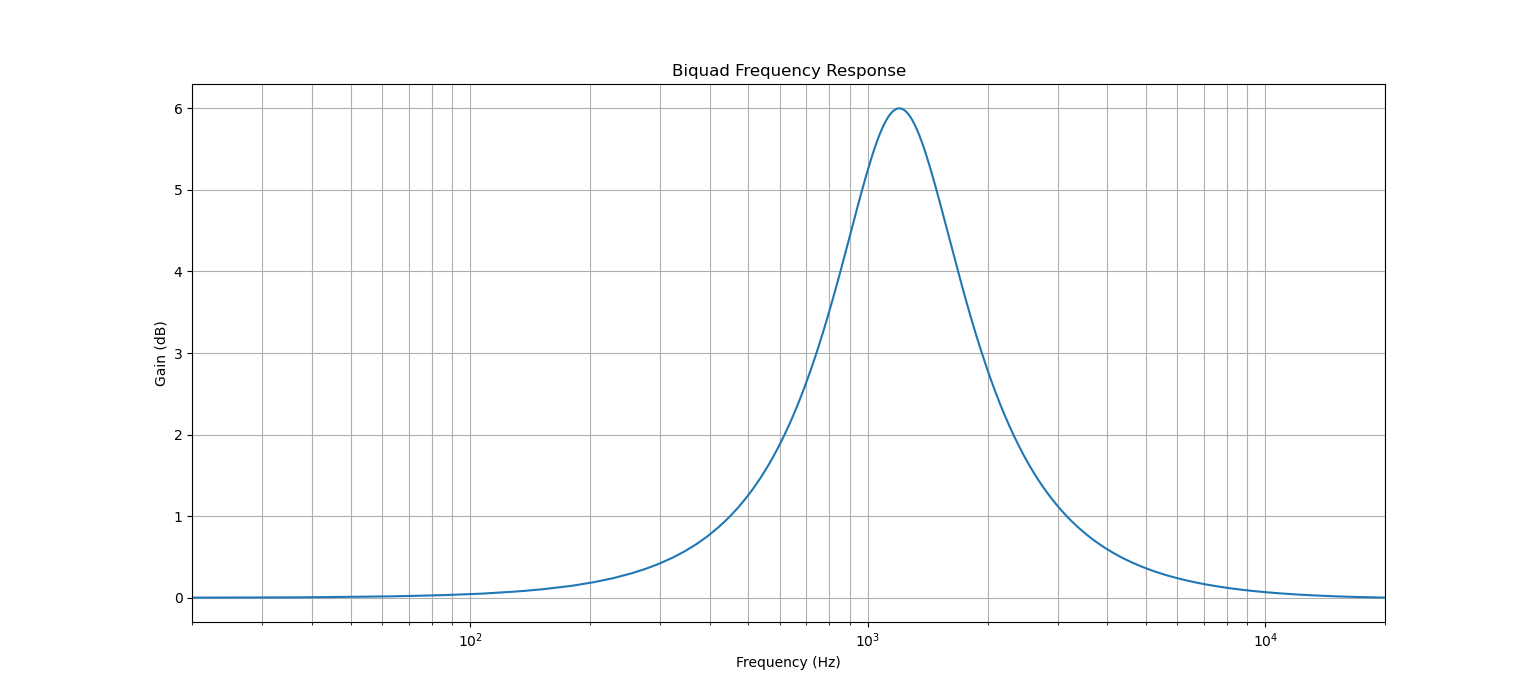
\includegraphics[width=\linewidth]{discussion/eq_filter/figures/rbj_bode_plot.png}
  \caption{Measured frequency Response from the RBJ Biquad Filter using Peaking EQ}
  \label{fig:rbj_bode_plot}
\end{figure}

Since this equation provides flexibility and a wide variety of shapes and sizes for each filter response
including peaking, shelving, low-pass, high-pass, notch, and band-pass responses,
Biquad filter is chosen for creating Parametric equalizers (\cref{prompt:parametric_eq}) \cite{openai_chatgpt,cookbook}, 
which are commonly used in many DAWs and VST Plugins \cite{fox2021parametriceq}.